\documentclass[tikz,border=12pt]{standalone}
\usetikzlibrary{arrows.meta,positioning,fit}
\definecolor{pink}{HTML}{F72585}\definecolor{blue}{HTML}{228BE6}\definecolor{green}{HTML}{2F9E44}
\definecolor{amber}{HTML}{F08C00}\definecolor{ink}{HTML}{343A40}\definecolor{soft}{HTML}{F1F3F5}
\begin{document}
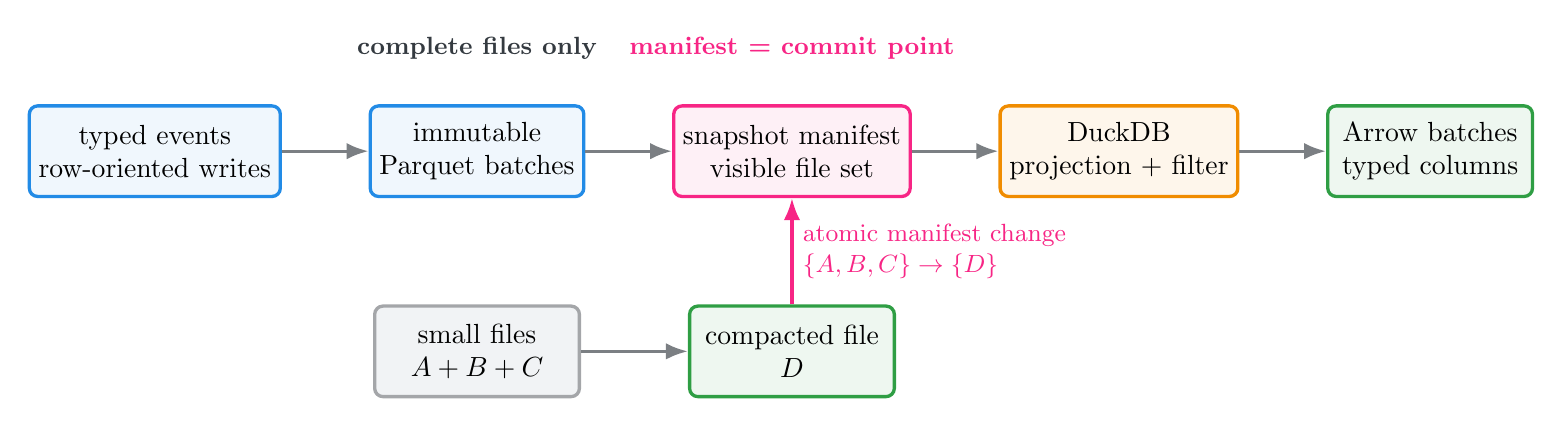
\begin{tikzpicture}[box/.style={rounded corners=3pt,draw=blue,fill=blue!7,very thick,minimum width=2.6cm,minimum height=1.15cm,align=center},arrow/.style={-{Latex[length=2.8mm]},very thick,ink!65},label/.style={font=\small\bfseries,text=ink}]
 \node[box] (events) {typed events\\row-oriented writes};
 \node[box,right=1.1cm of events] (batch) {immutable\\Parquet batches};
 \node[box,draw=pink,fill=pink!7,right=1.1cm of batch] (snapshot) {snapshot manifest\\visible file set};
 \node[box,draw=amber,fill=amber!8,right=1.1cm of snapshot] (duck) {DuckDB\\projection + filter};
 \node[box,draw=green,fill=green!8,right=1.1cm of duck] (arrow) {Arrow batches\\typed columns};
 \draw[arrow] (events)--(batch); \draw[arrow] (batch)--(snapshot); \draw[arrow] (snapshot)--(duck); \draw[arrow] (duck)--(arrow);
 \node[label,above=.45cm of batch] {complete files only};
 \node[label,above=.45cm of snapshot,text=pink] {manifest = commit point};
 \node[box,draw=ink!45,fill=soft,below=1.35cm of batch] (old) {small files\\$A+B+C$};
 \node[box,draw=green,fill=green!8,below=1.35cm of snapshot] (compact) {compacted file\\$D$};
 \draw[arrow] (old)--(compact);
 \draw[-{Latex[length=2.8mm]},very thick,pink] (compact)--node[right,font=\small,align=left]{atomic manifest change\\$\{A,B,C\}\to\{D\}$}(snapshot);
\end{tikzpicture}
\end{document}
